\documentclass[crop, tikz]{standalone}
\usepackage{tikz}

% Colour
\usepackage{xcolor}
\colorlet{LightCyan}{cyan!30}
\colorlet{LightLime}{lime!40}

% Nodes
\tikzstyle{LSTMblock}=[draw,fill=LightCyan,minimum size=20pt,inner sep=1pt]
\tikzstyle{invisNode}=[circle, line width=0mm, inner sep=0pt]
\tikzstyle{stateTransition}=[-stealth, thick]
\tikzstyle{dotted}=[line width=1pt, dash pattern=on \pgflinewidth off 6pt]
\tikzstyle{sumNode}=[draw,circle,fill=LightLime,minimum size=20pt,inner sep=1pt]


\begin{document}
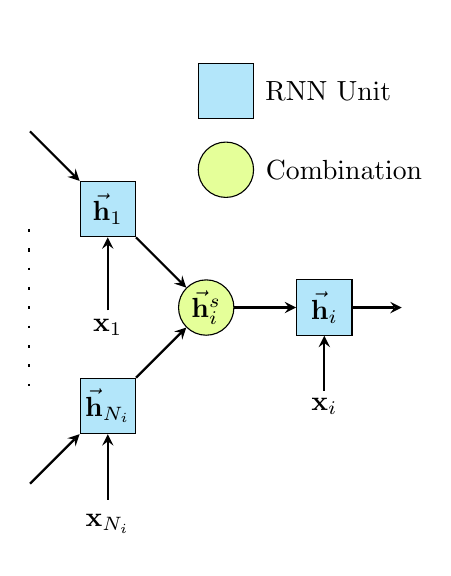
\begin{tikzpicture}
    % Incoming layer
    \node[invisNode] (invis1) at (-5.25,2.25) {};
	\node[LSTMblock] (h0) at (-4.25, 1.25) {$\vec{\mathbf{h}}_{1}$};
	\node[invisNode] (x0) at (-4.25, -0.25) {$\mathbf{x}_{1}$};
	\draw[stateTransition] (invis1) to[out=315,in=135] node [midway, sloped, above] {} (h0);
	\draw[stateTransition] (x0) to[out=90,in=270] node [midway, sloped, above] {} (h0);

    \node[invisNode] (invis2) at (-5.25,-2.25) {};
	\node[LSTMblock] (h1) at (-4.25, -1.25) {$\vec{\mathbf{h}}_{N_i}$};
	\node[invisNode] (x1) at (-4.25, -2.75) {$\mathbf{x}_{N_i}$};
	\draw[stateTransition] (invis2) to[out=45,in=225] node [midway, sloped, above] {} (h1);
	\draw[stateTransition] (x1) to[out=90,in=270] node [midway, sloped, above] {} (h1);

	\draw[dotted] (-5.25, 1.0) to[out=270,in=90] node [midway, sloped, above] {} (-5.25, -1.0);

    % Sum node
	\node[sumNode] (h2) at (-3, 0) {$\vec{\mathbf{h}}_i^s$};
	\draw[stateTransition] (h1) to[out=45,in=225] node [midway, sloped, above] {} (h2);
	\draw[stateTransition] (h0) to[out=315,in=135] node [midway, sloped, above] {} (h2);
	
	% Propagated forward state
	\node[LSTMblock] (h3) at (-1.5, 0) {$\vec{\mathbf{h}}_{i}$};
	\node[invisNode] (h4) at (-0.5, 0) {};
	\draw[stateTransition] (h2) to[out=0,in=180] node [midway, sloped, above] {} (h3);
	\draw[stateTransition] (h3) to[out=0,in=180] node [midway, sloped, above] {} (h4);
	\node[invisNode] (x2) at (-1.5, -1.25) {$\mathbf{x}_{i}$};
	\draw[stateTransition] (x2) to[out=90,in=270] node [midway, sloped, above] {} (h3);

    % Legend
    \node[LSTMblock] (LSTMLegend) at (-2.75,2.75) {};
    \node[invisNode] (LSTMtext) at (-1.45,2.75) {RNN Unit};
    \node[sumNode] (sumLegend) at (-2.75,1.75) {};
    \node[invisNode] (LSTMtext) at (-1.25,1.75) {Combination};

\end{tikzpicture}

\end{document}